\documentclass[12pt]{article}
\usepackage[a4paper,margin=.5in]{geometry}
\usepackage{graphicx}
\usepackage{booktabs}
\usepackage{listings}
\usepackage{color}

\definecolor{dkgreen}{rgb}{0,0.6,0}
\definecolor{gray}{rgb}{0.5,0.5,0.5}
\definecolor{mauve}{rgb}{0.58,0,0.82}

\lstset{frame=tb,
  language=Python,
  aboveskip=3mm,
  belowskip=3mm,
  showstringspaces=false,
  columns=flexible,
  basicstyle={\small\ttfamily},
  numbers=none,
  numberstyle=\tiny\color{gray},
  keywordstyle=\color{blue},
  commentstyle=\color{dkgreen},
  stringstyle=\color{mauve},
  breaklines=true,
  breakatwhitespace=true,
  tabsize=3
}
%\usepackage{subfig}
\usepackage{subcaption}
\usepackage{hyperref}
\hypersetup{
    colorlinks=true,
    linkcolor=blue,
    filecolor=magenta,      
    urlcolor=cyan,
    pdftitle={Overleaf Example},
    pdfpagemode=FullScreen,
    }
\newcommand*{\figuretitle}[1]{%
    {\centering%   <--------  will only affect the title because of the grouping (by the
    \textbf{#1}%              braces before \centering and behind \medskip). If you remove
    \par\medskip}%            these braces the whole body of a {figure} env will be centered.
}
\title{Homework 2 Writeup}

\author{Tylman Michael\\CSE 546 Machine Learning}
\date{2/4/2023}
%moderncv theme
\usepackage[utf8]{inputenc} 
\begin{document}
\maketitle{}
\section{Data Preprocessing}
Before beginning to work with this data, I decided to normalize it using a combination of a standard scaler and a normalizer. 
Doing this will effectively place all of the data points on an n-sphere centered at 0 with a radius of 1. I've found in the past
that this is a very effective normalization technique for classifiers in my own experience, and Dr. Frigui mentioned explicitly 
in class that this form of normalization historically performs well with this type of data that we are using.

\section{5-Fold Cross-Validation}

Starting off with the first bullet point on the assignment, I will cover the results of my 5-fold cross-validation. 
I utilized the seaborn package to plot the test/train curves for each model type, with the accuracy on the y axis and 
the appropriate attribute on the x-axis. I always use a full end-to-end pipeline for reproducibility, and for this assignment
it was much easier for me to name the x-axis "Attribute" for all items instead of naming them "C" for the SVM and Logistic
Regression classifiers, and "K" for the KNN classifier.

Each line plot shown in Figure 1 will show a thin dark line surrounded by a lighter area of the same color. The thin, dark line corresponds to 
the mean of the 5 folds, whereas the wider light area corresponds to the standard deviation of the 5 folds. The ScatterPlot
is an image of the mean training accuracy vs. validation accuracy for each attribute.




\begin{figure}
  \begin{subfigure}{.5\textwidth}
  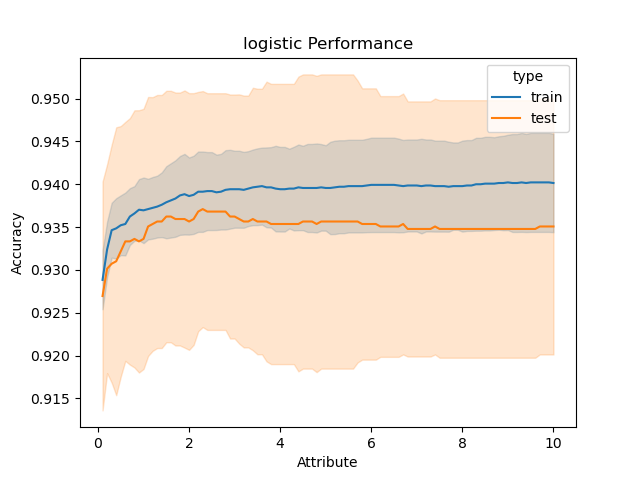
\includegraphics[width=.95\textwidth]{../results/logistic_Performance.png}
    \caption{Logistic Regression}
    \end{subfigure}%
  \begin{subfigure}{.5\textwidth}
    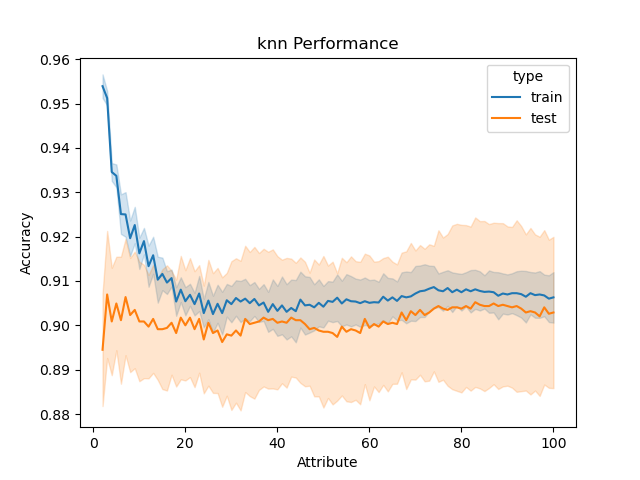
\includegraphics[width=.95\textwidth]{../results/knn_Performance.png}
    \caption{KNN}
    \end{subfigure}
  \begin{subfigure}{.5\textwidth}
    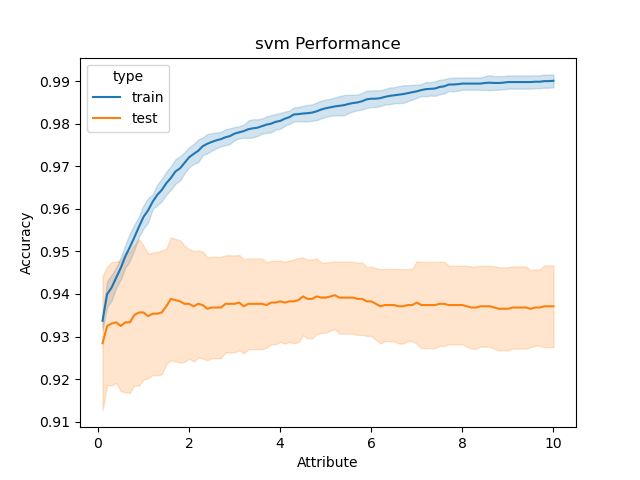
\includegraphics[width=.95\textwidth]{../results/svm_Performance.png}
    \caption{SVM}
  \end{subfigure}%
  \begin{subfigure}{.5\textwidth}
    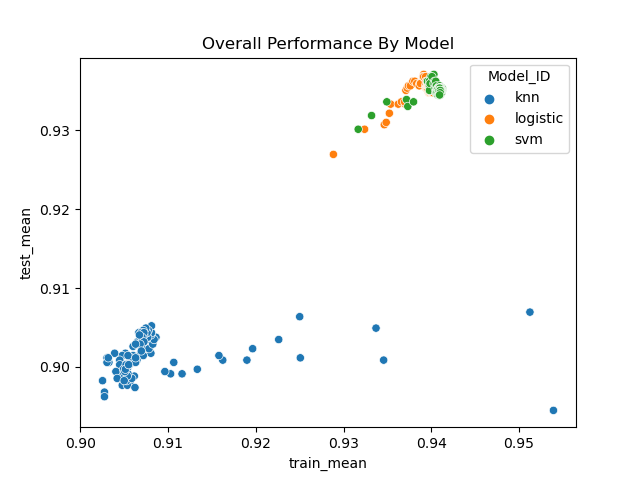
\includegraphics[width=.95\textwidth]{../results/Full_Scatter.png}
    \caption{Full ScatterPlot}
  \end{subfigure}
  \caption{KFold Cross-Validation Results}
  \label{figure1}
\end{figure}

\begin{table}
  \resizebox*{.95\textwidth}{!}{\begin{tabular}{llrrrrr}
\toprule
{} &  Model\_ID &  Attribute &  train\_mean &  train\_std &  test\_mean &  test\_std \\
\midrule
1   &       knn &        3.0 &    0.951232 &   0.001632 &   0.906957 &  0.014325 \\
121 &  logistic &        2.3 &    0.939130 &   0.004689 &   0.937101 &  0.013772 \\
210 &       svm &        1.2 &    0.940290 &   0.003295 &   0.937101 &  0.013267 \\
\bottomrule
\end{tabular}
}
  \caption{Best Results and MetaData}
  \label{table1}
\end{table}


\subsection{Optimal Parameters}
For each model, I simply took the max value for the mean test accuracy as my only criteria for selecting the optimal 
parameter. I think that criteria is sufficient for this stage in the class, though I am open to find more robust criteria 
for selection in future assignments.

The results of selecting the best attributes can be seen in Table \ref{table1}. For the KNN, the best model was the one with 3
Neighbors. For the  LR (Logistic Regressor), the best attribute was a $C=2.3$. Finally, for the SVM the best model was the one
with $C=1.2$ For all models, regardless of the attribute, the test standard deviation was significantly higher than the 
training std, which is to be expected.

For the Logistic Regression and SVM classifiers, they showed remarkable robustness to overfitting at all values, and underfitting
all the way until the performance began
to plateau out at a C value of about 4 and 2 respectively. After this point, we can see a bit of underfitting as the performance 
begins to dip slightly for training accuracy, and moderately for validation accuracy. Once we directly compare the two in Figure \ref{figure1}, we can see
that the Logistic Regressor showed slightly better overfitting because it had slightly better and more stable test accuracy, even with 
slightly less training accuracy across all attributes attempted.

I must admit to breaking my own rules a little bit on the KNN classifier. Normally, I do not like to include any manual 
pruning which is not repeatable from my pipeline, or to exclude results which meet my automated criteria.
However, this time I excluded the option of using 1 neighbor. I did so because it technically passed my criteria to be the 
best option for the KNN classifier, but it led to some uninteresting results later on and would likely lead to poor generalization
due to the clear possibility of overfitting. As such, I made the decision to remove that option from my analysis. 



\section{Final Test}
Once I selected the best parameters, I retrained a final model on the entirety of the training set, and applied it to the test 
set. The results of this can be found in Tabel \ref{table2}. Final\_Perf column is the final performance on the test set, and the 
Cval\_Perf column is the original performance on the test set cross-validation.

For all of these, the cross-validation performance was slightly better, which isn't unusual. The best performing item was the 
LR, which started off with the exact same test performance as the svm, but generalized better to lose less performance
on the test data. This would leave me to believe that the svm model is more prone to overfitting than the LR in 
this case.

The KNN and LR models suffered nearly identical loss of performance from Cval to Testing, but the LR
had notably better performance overall. This is an important note for the final conclusion.

\begin{table}
  \resizebox*{.95\textwidth}{!}{\begin{tabular}{lrr}
\toprule
   Model &  Attribute &  Final\_Performance \\
\midrule
     knn &        1.0 &           0.902693 \\
logistic &        2.3 &           0.925282 \\
     svm &        5.2 &           0.934839 \\
\bottomrule
\end{tabular}
}
  \caption{Final Test Results}
  \label{table2}
\end{table}

\section{Feature Analysis}
For the SVM and LR, I plotted the magnitude of the coefficients for each feature into Figure \ref{figure2}. These images are 
a little bit too tight, so I also included the top 5 features in Tables \ref{table3} and \ref{table4}. As we can see in these
tables, these methods share 4 of their top 5 features. Unfortunately, I am unfamiliar with what these features fully mean
so I can't draw many conclusions, but we can at least appreciate the consistency of our linear methods.

\begin{figure}
  \begin{subfigure}{.5\textwidth}
  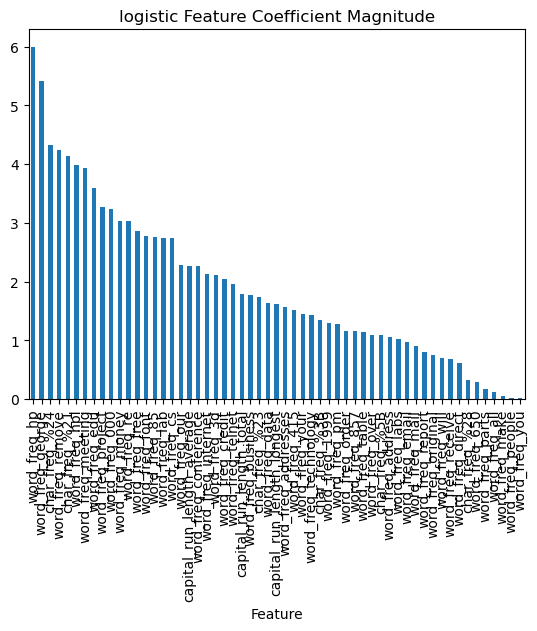
\includegraphics[width=.95\textwidth]{../results/logistic_features.png}
    \caption{Logistic Regression}
    \end{subfigure}%
  \begin{subfigure}{.5\textwidth}
    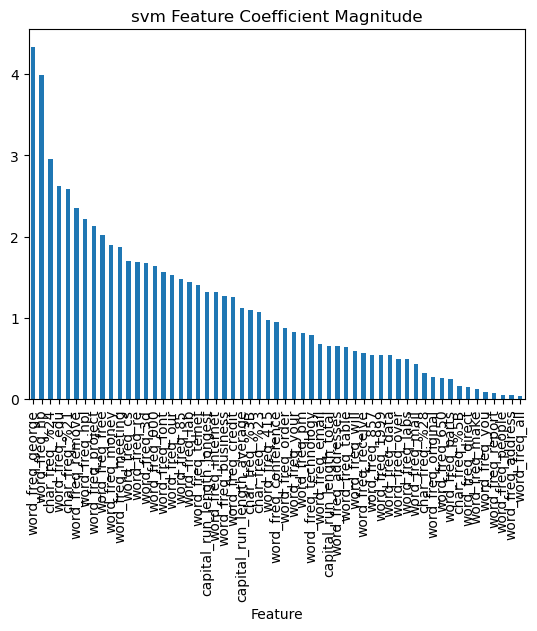
\includegraphics[width=.95\textwidth]{../results/svm_features.png}
    \caption{SVM}
  \end{subfigure}
  \caption{Feature Importance}
  \label{figure2}
\end{figure}

% \begin{figure}
%   \begin{subfigure}{.5\textwidth}
\begin{table}
  \parbox{.5\textwidth}{
    \begin{tabular}{lr}
\toprule
{} &  Importance \\
Feature          &             \\
\midrule
word\_freq\_george &    4.331504 \\
word\_freq\_hp     &    3.990053 \\
char\_freq\_\%24    &    2.951851 \\
word\_freq\_edu    &    2.625116 \\
char\_freq\_\%21    &    2.582081 \\
\bottomrule
\end{tabular}

    \caption{SVM Features}
    \label{table3}}
  % \end{subfigure}%
  % \begin{subfigure}{.5\textwidth}
    \parbox{.5\textwidth}{
      \begin{tabular}{lr}
\toprule
{} &  Importance \\
Feature          &             \\
\midrule
word\_freq\_hp     &    5.992098 \\
word\_freq\_george &    5.422156 \\
char\_freq\_\%24    &    4.333599 \\
word\_freq\_remove &    4.243031 \\
char\_freq\_\%21    &    4.137998 \\
\bottomrule
\end{tabular}

      \caption{LR Best Features}
      \label{table4}}
\end{table}
%   \end{subfigure}
%   \caption{Features}
%   \label[figure3]
% \end{figure}

\section{Missed Item Analysis}
The assignment also requested an analysis of a few misclassified samples. Unfortunately, I am not familiar enough with the 
data to meaningfully interact with missed samples and give a manual analysis, so I opted to perform a couple plotting endeavors.

First, I plotted a 3D interactive plot (included in supplements I will attempt to provide) to identify missclassified samples 
which appeared interesting. I chose one false positive sample and one false negative sample for analysis.
I've included screenshots of the two samples I chose in Figure \ref{figure3} in case I cannot upload my html files for you 
to access the original 3D plots.

As you can see in the plots, I chose the two samples which were most closely clustered with correctly identified samples. In 
the displayed information, we can see the name as the index in the training data, the truth value, the knn score, LR score, and 
the svm score.

Once I chose the two samples, I performed a UMAP transformation fit on the training data, and plotted these two samples into 
the transformed data. I also did this in 3D to get more practice with plotting in 3D. Once again, I will provide a screenshot 
of zoomed in results for you here in \ref{figure4} in case you cannot access my html files. 

In figure 4, blue dots belong to Safe items, red dots belong to Spam items, the green dot is the False Positive (FP) test sample, and 
the purple dot is the False Negative(FN) sample. In these plots, we can see that these samples are both clustering in an area of 
high amounts of the correct type (The FP sample is surrounded by Negative samples, and the FN is surrounded primarily by Positive samples);
however, both of these regions have a small amount of samples which belong to the other type as well. 

Personally, I don't think that this is enough evidence to explain solidly why all 4 of our models got this answer wrong. 
After some thought, I figured the issue was that I was using a nonlinear function to troubleshoot the behavior of a set of primarily linear 
classifiers, so I tried to do a linear projection using the SVD. Once I did this, I saw an impossible amalgamation of dots 
which provided no significant information for us, so I did not decide to continue pursuing this direction.

After I completed these steps, I decided I had done enough for the complexity requirement of this assigment, and decided to leave it at 
a more simple conclusion that these samples belong to an area of only mild heterogeneity between the classes, which require a 
classifier more complex than a linear classifier in order to capture the behavior of these outliers.


\begin{figure}
  \begin{subfigure}{.5\textwidth}
  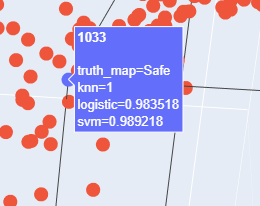
\includegraphics[width=.95\textwidth]{../results/False_Positive.png}
    \caption{False Positive Choice}
    \end{subfigure}%
  \begin{subfigure}{.5\textwidth}
    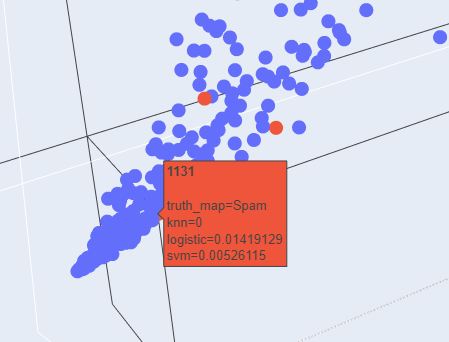
\includegraphics[width=.95\textwidth]{../results/False_Negative.png}
    \caption{False Negative Choice}
  \end{subfigure}
  \caption{Missed Sample 3D screenshots}
  \label{figure3}
\end{figure}

\begin{figure}
  \begin{subfigure}{.5\textwidth}
  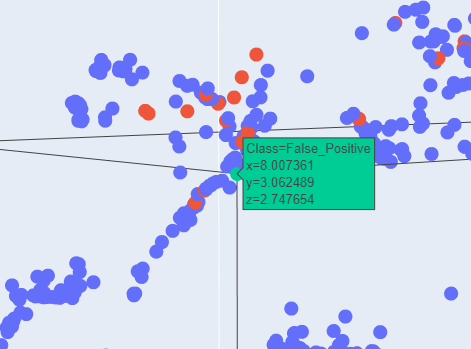
\includegraphics[width=.95\textwidth]{../results/False_Positive_UMAP.png}
    \caption{False Positive Choice}
    \end{subfigure}%
  \begin{subfigure}{.5\textwidth}
    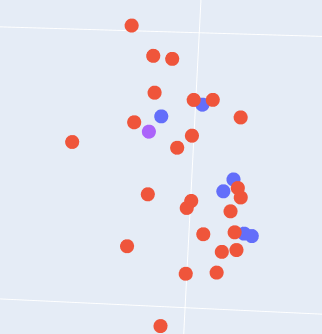
\includegraphics[width=.95\textwidth]{../results/False_Negative_UMAP.png}
    \caption{False Negative Choice}
  \end{subfigure}
  \caption{UMAP Transformation}
  \label{figure4}
\end{figure}

\section{Conclusion and Model selection}
I would have to choose the logistic regressor as the best algorithm for this dataset. It was tied for best accuracy for cross-validation,
had the best test accuracy, showed the best generalization, and is a standard and commonly understood classifier. Overall,
the Logistic Regression classifier clearly is the best choice out of these 3 options.

I know the 
assignment recommended including a discussion of time required to train/test, but honestly all of these simpler functions are so 
easy to train that I was able to train 100 models of each type (300 total) in a manner of minutes. As such, I struggle to think of 
an application where someone would need to ad-hoc train new models so quickly that the gain in time complexity would be worth losing
any of the above qualities that the Logistic Regressor showed to be the best at. 

With this in mind, my vote for the best model is the Logistic Regressor.


\end{document}